%! TEX root = **/010-main.tex
% vim: spell spelllang=en:

\section{Context and scope}%
\label{sec:context}

\subsection{Introduction and contextualization}%
\label{sub:intro}

Since its release in 2007, Compute Unified Device Architecture (CUDA) has
revolutionized the usage of graphic processing units for scientific
computations, allowing developers to implement programs that take full advantage
of the parallelization capabilities of GPUs for general purpose programming.
This paired with the exponential growth of computing power that GPUs have
experienced in the last decade has made GPU numerical analysis essential on
modern science research. Highly complex problems that where once impossible to
compute in realistic time frames can now be computed even on average consumer
hardware GPUs. Moreover, projects like
\emph{GPUGRID}\footnote{\url{www.gpugrid.net}} allow researches to run
distributed programs through a grid of GPUs from volunteers all over the world
reaching supercomputing level performance \cite{antaviana_nvidia_nodate}.


In 1900 David Hilbert posed a list of 23 problems in the field of mathematics
which were unsolved at the time \cite{hilbert_mathematische_1900}.  Those
problems have been vastly studied since then and most of them are solved or
partially solved. There are however some which are still unsolved to this day.

One of these unsolved problems is the 16th problem.  This problem consists of
two separate problems, the first one regarding the relative positions of the
branches of real algebraic curves and the second one about the upper limit of
limit cycles on two dimensional vector fields and their relative positions. In
this project we are going to study the second part of this 16th problem.

In particular, we study the number of limit cycles for vector fields of
polynomials of second degree:

\begin{align}
    \frac{dx}{dt} &= a_1x^2 + b_1xy + c_1y^2 + \alpha_1x + \beta_1y \\
    \frac{dy}{dt} &= a_2x^2 + b_2xy + c_2y^2 + \alpha_2x + \beta_2y
\end{align}

It's unknown whether there exists an upper limit on the number of limit cycles
for systems with polynomials of degree greater than one
\cite{ilyashenko_centennial_2002}.


% todo
% Determining if a point is part of a limit cycle is shown to be
% \textbf{PSPACE}-complete  \cite{papadimitriou_computational_2015}


\subsubsection{Context}

This is a Bachelor Thesis of the Computer Engineering Degree, specialization in
Computing, done in the Facultat Inform\`atica de Barcelona (FIB) of the
Universitat Polit\'ecnica de Catalunya (UPC). The project is directed by Grigori
Astrakharchik.

\subsubsection{Concepts}

Below are some concepts needed to understand the project.

\newcommand{\concept}[1]{\textbf{#1}\\}

% \concept{Ordinary differential equations}
%todo

\concept{Limit cycles}
A limit cycle is a closed trajectory with the property that at least one other
trajectory spirals into it as time approaches infinity. They are important in
various applications in the field of dynamical systems.

\concept{CUDA}
CUDA is a parallel computing platform developed by \emph{nvidia} that allows general
computing on their graphic processing units (GPUs). Using the CUDA programming
model allows developers to run massively parallel programs on GPUs.

\subsubsection{Problem to be solved}

There have been various studies on the number of limit cycles for second degree
vector fields but so far the maximum number of cycles found is 4
\cite{kuznetsov_visualization_2013}. The aim of this project is to search the
parameter space for systems that have 4 or more cycles to gain more insight on
the nature of these equations.

\Cref{fig:kuznetsov} shows a visualization of the limit cycles of a
two-dimensional polynomial quadratic system.

\begin{figure}[H]
    \centering
    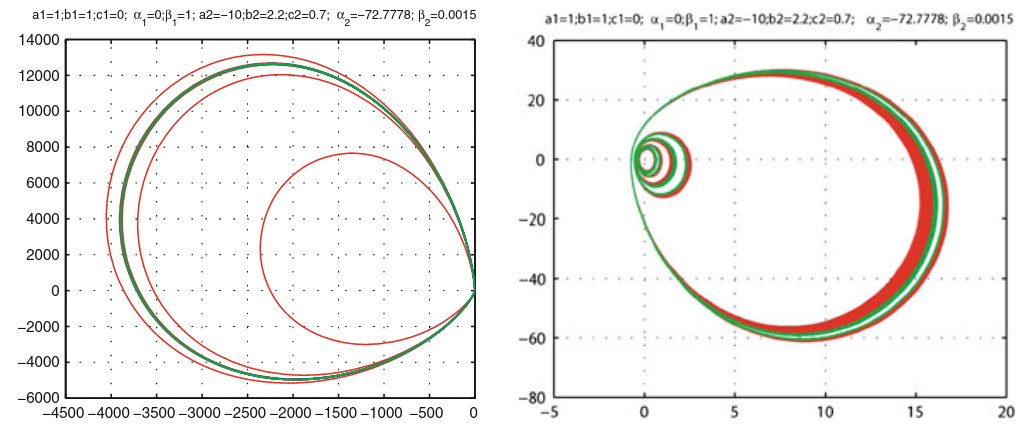
\includegraphics[width=1.0\textwidth]{4cycles}
    \caption{Visualization of four limit cycles in two-dimensional polynomial quadratic system
        \cite{kuznetsov_visualization_2013}
    }%
    \label{fig:kuznetsov}
\end{figure}

To do so, we'll implement a parallel algorithm that solves ODE systems and
detects limit cycles for a wide range of parameters and points in the plane.
This code will be implemented in Julia programming language and will use CUDA
to be able to run it in the GPUs at the Minotaur cluster from the BSC.

\subsubsection{Stakeholders}



\subsection{Justification}
\subsubsection{Previous studies}

As stated before there have been numerous studies on the field of limit cycles.
Kuznetsov et al. showed some conditions for which 4 limit cycles can be found
\cite{kuznetsov_visualization_2013}.

Papadimitriou and Vishnoi showed that the computation of a limit cycle is
\textbf{PSPACE}-complete \cite{papadimitriou_computational_2015}

And there have been some studies on numerical methods to find limit cycles on
two dimensional vector fields
\cite{leonov_hidden_2013,van_der_hoff_numerical_2013,casades_computation_2013,gasull_effective_nodate}

There are various programing languages with libraries for CUDA programming.
The official CUDA programming model is in C/C++ and offers the most flexibility
and performance. The other two most notable alternatives are Python's Numba
and Julia's CUDA.jl, these libraries are higher level and don't offer the same
low level options but allow easier development and visualization of the data.
Both use the official CUDA C interface under the hood so although the
performance as good as with pure C its comparable since the majority of the work
is done in the CUDA kernels anyways. Since Julia JIT compilation is faster than
python and provides similar advantages when visualizing data the initial idea is
to program the whole project in Julia programming language.

This is not a strict constraint and the possibility of writing specific C CUDA
code to tweak the performance to the maximum will be studied.

% todo


\subsection{Scope}
\subsubsection{Objectives and sub-objectives}

The main objective of this thesis is to develop a highly efficient program
capable of determining the possible existence of limit cycles for a system. This
program must also be capable of being executed in parallel in a GPU making full
use of its computing power to analyze a wide variety of systems with different
parameters. Furthermore the results must be evaluated to find interesting
systems to visualize and analyse in more detail. These objectives can be divided
in sub-objectives:

\paragraph{Theoretical part} Before implementing the program a deep
understanding of the current numerical methods and the CUDA framework must be
analysed to find the best approach to the problem.

\begin{itemize}
    \item Explore numerical methods to compute ordinary differential equations.
    \item Explore numerical methods to evaluate the existence of limit cycles
        and determine the number of cycles for a given system.
    \item Research how these methods can be applied to run in a CUDA system
        efficiently.
\end{itemize}

\paragraph{Practical part} Having done the background research, the code must be
implemented possibly trying different methods to find the ones that give the
best results in practice.

\begin{itemize}
    \item Program the studied methods
    \item Benchmark the performance and try different approaches to achieve the
        best performance.
    \item Run the code.
    \item Analyze the results and visualize them.
\end{itemize}

\subsubsection{Requirements}

To ensure the quality of the thesis some requirements must be fulfilled:

\begin{itemize}
    \item Find the best balance between accuracy of the results and
        computational complexity
    \item Ensure that the numerical methods applied are properly implemented.
    \item Take into account numerical stability of the method used as well as
        rounding and overflow errors.
    \item Profile the different methods under the same conditions and
        environment to ensure that there are no biases.
    \item Use good programming practices, making readable and maintenable code with the least
        complexity possible.
\end{itemize}

\subsubsection{Potential obstacles and risks}

There are several risks that may have to be dealt with during the development
of this thesis.

\begin{itemize}
    \item \textbf{Project deadlines}: There is a limited amount of time to
        do the project. Therefore a proper planning of tasks and time must be
        made and followed to ensure that the work can be done in the proper
        timeframe.
    \item \textbf{Computational power}: This thesis involves a lot of
        computing power and it's conditioned by it. If the program cannot be run
        on the proper hardware the results may not be obtainable in a realistic
        timeframe and the scope of the project will have to be reevaluated.
    \item \textbf{Inexperience on the field}: I have very limited experience
        with CUDA programming and just the basics of numerical computation
        techniques so there is a lot of research to be done. Specially regarding
        dynamical systems.
\end{itemize}

\subsection{Methodology and rigor}

\subsubsection{Methodology}

Since the thesis must be completed in a relatively short period of time we will
apply the \emph{agile} methodology and divide the work into subtasks or
\emph{sprints}. These \emph{sprints} will consist of different stages of
implementation of the program, beginning with a proof of concept running in
sequence on the CPU and progressively iterating on this base to optimize the
methods and adapt them to be able to run in CUDA on the GPU.

\subsubsection{Monitoring tools and validation}

To manage the different iterations of the code \texttt{git} will be used. The
repository will be hosted on \emph{GitHub} and access will be granted to the
project tutor allowing him to follow and monitor the work and results at any time.

A weekly meeting with the tutor will be arranged to discuss the progress and
which tasks should be worked on.
